\documentclass[12pt,twocolumn]{article}
\usepackage[margin=1.5cm]{geometry}
\usepackage{amsmath}
\usepackage{graphicx}
\usepackage{hyperref}
\title{RLC circuits and AC Sources}
\author{Prof. Jordan C. Hanson}

\begin{document}
\small
\maketitle

\section{Introduction}

\begin{figure}[ht]
\centering
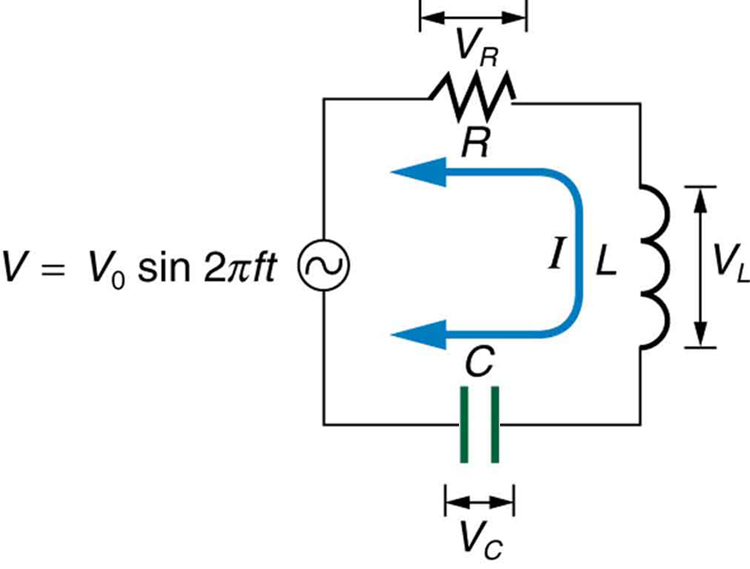
\includegraphics[width=0.35\textwidth]{RLC_1.jpeg}
\caption{\label{fig:rlc_1} \textit{Series RLC circuits} have a resistor $R$, an inductor $L$, and a capacitor $C$.  In this example, the AC voltage source drives current in the circuit sinusoidally.}
\end{figure}

\noindent
In this lab activity, we will build upon our experience gained with the RLC PhET simulation.  Within the simulation, we modeled a series RLC circuit and located the \textit{resonance frequency}, $f_0$:
\begin{equation}
f_0 = \frac{1}{2\pi\sqrt{LC}}
\end{equation}
Another important result from RLC circuit theory is the \textit{bandwidth} of the resonance.  Let $f_0$ be the resonance frequency, with 100\% AC circuit power.  Let $f_1$ and $f_2$ be the two frequencies above and below resonance that correspond to 50\% AC circuit power.  We define bandwidth as $\Delta f = f_2 - f_1$, and it may be shown that
\begin{equation}
\frac{\Delta f}{f_0} = R\sqrt{\frac{C}{L}}
\end{equation}
That is, a larger $R$ corresponds to higher bandwidth.  In AM radio receivers, the value of $R$ controls how \textit{selective} the receiver is.  If the value of $R$ is too large, multiple radio stations will be received.  If the value of $R$ is too small, only the carrier (and not the audio modulation) will be received.

\section{Experimental Setup}

\noindent
Check that you have the following items at your table:
\begin{itemize}
\item The Analog Arts USB-powered oscilloscope and signal generator unit
\item A 6-foot USB cable to connect the Analog Arts unit to the desktop PC
\item The Analog Arts application on the PC desktop
\item Two BNC to probe-clip coaxial cables
\item One 100 $\mu$H inductor, and one 0.1 $\mu$F capacitor
\item A wire with alligator clip connectors
\item A digital voltmeter set to measure resistance.
\end{itemize}

Click on the Analog Arts icon on the PC desktop window.  After a calibration stage, the application should launch.  From the list of functions, choose the oscilloscope.  We should recall the controls from the lab activity involving Faraday's Law and Mutual Inductance.  For example, recall the function of the Volts/division and microseconds/division controls.  Recall the function of the \textit{trigger}, represented by an arrow on the left vertical axis.  The trigger can activate on a \textit{rising edge}, or a \textit{falling edge.}  Normal trigger mode means we are in control of the threshold, and no signal will be drawn unless our trigger is satisfied.  With auto mode enabled, signals will be drawn asynchronously.

Connect a BNC cable to the signal generator output on the Analog Arts unit.  Now connect the \textbf{red} probe connector to one side of the inductor.  Connect the wire with alligator clip to the other side of the inductor.  Connect the wire to one side of the capacitor.  Connect the \textbf{black} BNC probe connector to the other side of the capacitor.  The RLC circuit is now closed.  The $R$ needs to be small for this lab activity, and the combined resistance of the wire and inductor is sufficient.  Activate the arbitrary waveform generator option in the Analog Arts program, and choose a sinusoidal signal with a 1kHz frequency and 1 Vpp amplitude.   Connect the other BNC cable to the channel 1 input on the Analog Arts unit, and connect the probes across the capacitor.  Activate the oscilloscope option in the Analog Arts application, and adjust the trigger settings until the sinusoidal signal is located.

\section{Data Collection and Error Analysis}

Set the voltmeter to measure Ohms, on the lowest setting ($200$ $\Omega$).  Temporarily disconnect the inductor and wire from the series RLC setup to make the measurement of total resistance.  Measure the total resistance of the wire and inductor, and record your result here: \\ \vspace{0.5cm}

\underline{$R\pm \sigma_R: ~~~~~ \pm ~~~~~$} $\Omega$. \\ \vspace{0.5cm}

Because the fractional error in $R$ likely exceeds that of $L$ or $C$, we will neglect errors in $L$ and $C$.  The error propagation of $R$ to the bandwidth ratio $r = \Delta f/f_0$ is

\begin{equation}
\sigma_r = \sigma_R \sqrt{\frac{C}{L}} \label{eq:error}
\end{equation}

Equation \ref{eq:error} is simply that the fractional error in $r$ is equal to the fractional error in $R$ if we neglect errors in $L$ and $C$ ($\sigma_r/r = \sigma_R/R$).  Further, if we neglect errors in $L$ and $C$, this means we are assuming no error in $f_0$, since $f_0$ depends only on $L$ and $C$.  Using the values of $R$, $L$, and $C$, make predictions of $f_0$ and $r = \Delta f/f_0$ below. \\ \vspace{0.5cm}

\underline{$f_0: ~~~~~~~~~~$} kHz, and \underline{$r \pm \sigma_r: ~~~~~~~~~~\pm~~~~~~~~~~$} \\ \vspace{0.5cm}

Adjust the frequency of the AC voltage in kHz to observe changes in the amplitude of the channel 1 signal.  Note that you will have to adjust the trigger, volts/division, and time/division controls.  For the frequencies in Tab. \ref{tab:data}, record the channel 1 amplitude.  Enter the data from Tab. \ref{tab:data} into a spreadsheet.  Create a graph of AC voltage frequency versus channel 1 amplitude.  Draw a scientifically accurate versions of these graphs in the space below Tab. \ref{tab:data}. \\ \\ \\

\begin{table}[ht]
\footnotesize
\begin{tabular}{| c | c |}
\hline
\textbf{AC voltage freq.} [kHz] & \textbf{Channel 1 amp.} [mV] \\ \hline
48.2 & \\ \hline
48.5 & \\ \hline
48.8 & \\ \hline
49.1 & \\ \hline
49.4 & \\ \hline
49.7 & \\ \hline
50.0 & \\ \hline
50.3 & \\ \hline
50.6 & \\ \hline
50.9 & \\ \hline
51.2 & \\ \hline
51.5 & \\ \hline
51.8 & \\ \hline
52.1 & \\ \hline
52.4 & \\ \hline
\end{tabular}
\caption{\label{tab:data} Perform the necessary measurements to complete this table.}
\end{table}

\noindent
\textbf{AC Voltage Freq, vs. Channel 1 Amp.:} \\ \\ \\ \\ \\ \\ \\ \\ \\ \\

\section{Analysis and Discussion}

Answer the quesions below Fig. \ref{fig:rlc_2}.

\begin{figure}[ht]
\centering
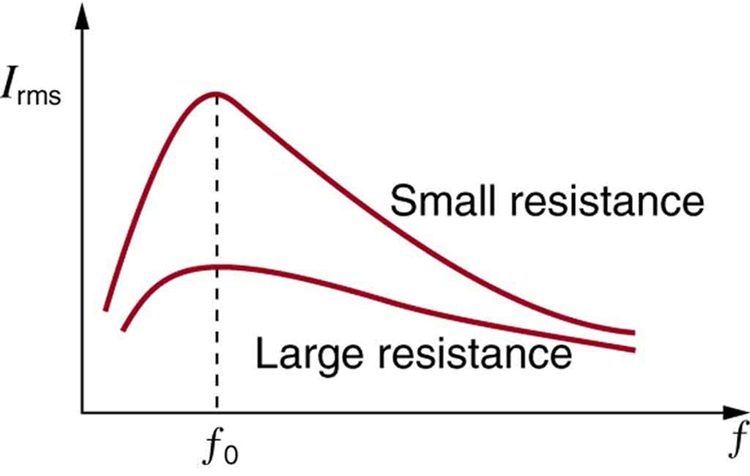
\includegraphics[width=0.5\textwidth]{RLC_2.jpeg}
\caption{\label{fig:rlc_2} A resonance curve for an RLC circuit.}
\end{figure}

\begin{enumerate}
\item Do you observe the predicted resonance frequency?
\item On your plot above, the \textit{bandwidth} is the frequency range $\Delta f$ over which the amplitude decreases by $1/\sqrt{2}$.  This corresponds to a factor of 2 decrease in power (50\% power).  Measure $\Delta f$ and divide by $f_0$ to obtain the ratio $r$ (the fractional bandwidth).  Does this result match your prediction?
\item Your graph should resemble Fig. \ref{fig:rlc_2}, near the peak.  Is this the case?
\end{enumerate}

\end{document}